\section{Method Overview}
\label{sec:method}
\subsection{Problem Statement}
Given series of point sets which record the same group of rigid indoor objects with different layout. We intend to samutaneously partition the point sets into objects and align the points of same object to recover layouts for corresponding object. Figure~\ref{fig:teaser} shows an example of input point clouds set.
\subsection{Basic Formulation}
To simutaneously model the joint registration and co-segmentation,  we come up with a generative model as follows:
\begin{equation}
\label{equ:model}
P(v_{mi})=\sum^{K_n}_{k=1}p_kN(v_{mi}|\phi_{mn}(x_k),\Sigma_k)
\end{equation}
which treat the i-th observed point $v_{mi}$ from the m-th point set as a sample point generated by one of $N$ object models.
We can define:\\
$$\Theta=\{\{p_k,x_k,\Sigma_k\}_{k=1}^{\sum{K_n}},\{\phi_{mn}\}_{m=1,n=1}^{MN}\}$$
as the parameter set of the generative model.\\
$p_k$ is the weight of the k-th Gaussian.\\
$x_k$ is the center of the k-th Gaussian.\\
$\Sigma_k$ is the standard deviation of the k-th Gaussian.\\
There are $K_{all}=\sum{K_n}$ Gaussian models in total and among them $K_n$ Gaussian models are treated as a group to represent n-th object.\\
$V$ is the set of M input point sets.\\
$v_{mi}$ is the i-th point of the m-th point cloud.\\
$\{\phi_{mn}\}$ are the functions of rigid transformation that transform the n-th group of gaussian centroids (representing the n-th object ) to the space of m-th input point sets.\\ 
Each object model is represented by a group of $K_n$ gaussian models.\\
Our goal of optimization is to maximize the probability of observed input sets sampled from the latent model.This problem can be solved in the framework of expectation-maximization. In particular, we bring in a latent parameter\\
$$Z=\{z_{mn}|m=1...M,n=1...N_m\}$$
such that $z_{mn}=k(k=1...\sum{K_n})$ assigns the observed point $v_{mi}$ to the k-th component of Gaussian mixture model. We aim to maximize the expected complete-data log-likelihood:
\begin{equation}
\label{equ:obj0}
f(\Theta|V,Z)=\mathbb{E}_Z[\ln P(V,Z;\Theta)|V]
\end{equation}
The object can be written as:
\begin{equation}
\label{equ:obj1}
\Theta=\arg\max{\sum_ZP(Z|V,\Theta)\ln{P(V,Z;\Theta)}}
\end{equation}
Such formulation can be seen as an adaption of joint registration formulation in \cite{Evangelidis2014}, upon which we seperate Gaussian models into groups to express multiple objects and the latent parameter  $Z$ that assign observed points to gaussian models can naturally indicate the object level segmentation.\\
By the asssumption of independent and identically distributed of input points, we can write the objective to:
\begin{equation}
\label{equ:obj2}
\Theta=\arg\max\sum_{mik}\alpha_{mik}(\ln p_k + \ln P(v_{mi}|z_{mi}=k;\Theta))
\end{equation}
where $\alpha_{mik} = P( z_{mi} = k | v_{mi} ; \Theta )$\\
By bringing in equation \ref{equ:model} and ingnoring constant terms, we can rewrite the objective as:
\begin{equation}
\label{equ:obj3}
\Theta=\arg\max\sum_{mik}\alpha_{mik}(||v_{mi}-\phi_{mn}(x_k)||_{\Sigma_k}^2 + \ln |\Sigma_k| - 2\ln p_k)
\end{equation}
where the $|\cdot|$ denotes the determinant and $||x||_A^2=x^TA^{-1}x$. It is predefined that $x_k$ is one of the gaussian centroid used to represent n-th object, which is why we apply transformation $\phi_{mn}$ on to the $x_k$. For the convenience of computation, we restrict the model to isotropic covariances, i.e.,$\Sigma_k=\sigma^2I$ and $I$ is the identity matrix.\\
Now, we can optimize this through iterating between estimating $\alpha_{mik}$ (Expectation-step) and maximizing $f(\Theta|V,Z)$ sequentially with respect to each parameters in $\Theta$ (Maximization-steps).
These steps are:\\
\textbf{E-step}:
this step estimates the posterior probability $\alpha_{mik}$ of $v_{mi}$ to be a point generated by the k-th Gaussian model.\\
\begin{equation}
\label{equ:estep}
\alpha_{mik}=\frac{p_k\sigma_k^{-3}exp(-\frac{1}{2\sigma_k^2}||v_{mi}-\phi_{mn}(x_k)||^2)}{\sum_s^{K_{all}}p_s\sigma_s^{-3}exp(-\frac{1}{2\sigma_s^2}||v_{mi}-\phi_{mn}(x_s)||^2)}
\end{equation}
\textbf{M-step-a}:this step update the transformations $\phi_{mn}$ that maximize $f(\Theta)$, given instant values for $\alpha_{mik}$, $x_k$, $\sigma_k$. We only consider rigid transformations, making  $\phi_{mn}(x)=R_{mn}x+t_{mn}$. The maximizer $R_{mn}^*,t_{mn}^*$  of $f(\Theta)$ is the same with the minimizers of the following constrained optimization problems:\\
\begin{equation}
\left\{
\begin{array}{rcl}
\min_{R_{mn},t_{mn}}&      &||(W_{mn}-R_{mn}X_n-t_{mn}\mathbf{e}^T)\Lambda_{mn}||_F^2\\
s.t.&      &R_{mn}^TR_{mn}=I, |R_{mn}|=1\\
\end{array} \right.
\end{equation}
where $\Lambda_{mn}$ is $K_n \times K_n$ diagonal matrix with elements $\lambda_{mnk}=\frac{1}{\sigma_k}\sqrt{\sum_i^{I_{m}}\alpha_{mik}}$,$I_m$ is the number of point for the m-th input point set, $X_n = [x_1,x_2,....,x_{K_n}]$ is the matrix stacked by the centroids of gaussian models that are predefined to represent the n-th object. $\mathbf{e}^T$ is a vector of ones, $||\cdot||_F$ denotes the Frobenius norm, and $W_{mn}=[w_{m1},w_{m2},...,w_{mk},...,w_{mK_n}]$, in which $w_{mk}$ is a weighted point as:\\
\begin{equation}
w_{mk}=\frac{\sum_{i=1}^{I_m}\alpha_{mik}v_{mi}}{\sum_{i=1}^{I_m}\alpha_{mik}}
\end{equation}
This problem have a similar solution of in \cite{Evangelidis2014}. The only difference is that we are estimating the transformation from latent models to the input point sets, since there are multiple group of $x_k$ corresponding to multiple objects in our latent model. The optimal can be given by:\\
\begin{equation}
R_{mn}^*=U_{mn}C_{mn}V_{mn}^T
\end{equation}
\begin{equation}
t_{mn}^*=\frac{1}{tr(\Lambda_{mn}^2)}(W_{mn}-R_{mn}X_n)\Lambda_{mn}^2\mathbf{e}
\end{equation}
where $[U_{mn},S,V_{mn}]=svd( W_{mn}\Lambda_{mn}P_{mn}\Lambda_{mn}X_{mn}^T )$ and $P_{mn}=I-\frac{\Lambda_{mn}\mathbf{e}(\Lambda_{mn}\mathbf{e})^T}{(\Lambda_{mn}\mathbf{e})^T\Lambda_{mn}\mathbf{e}}$,$I$ is identity matrix. $C_{mn}=diag(1,1,|U_{mn}||V_{mn}|)$.\\
\textbf{M-step-b}: this step we update the parameters related to the Gaussian mixture model. 
\begin{equation}
x_k^*=\frac{\sum_{m=1}^M\sum_{i=1}^{I_m}\alpha_{mik}(R_{mn}^{-1}v_{mi}-t_{mn})}{\sum_{m=1}^M\sum_{i=1}^{I_m}\alpha_{mik}}
\end{equation}
where $x_k$ is one of the Gaussian centroids that is predefined to represent n-th object. 
\begin{equation}
\sigma_k^{*2}=\frac{\sum_{m=1}^M\sum_{i=1}^{I_m}\alpha_{mik}||(v_{mi}-t_{mn}-R_{mn}^*x_k^*)||_2^2}{3\sum_{m=1}^M\sum_{i=1}^{I_m}\alpha_{mik}}
\end{equation}
\begin{equation}
p_k^*=\frac{\sum_{m,i}\alpha_{mik}}{M}
\end{equation}
\subsection{Bilateral Formulation}
When considering features, we can add bilateral terms into the generative model.
\begin{equation}
P(v_{mi},f_{mi})=\sum^{K_n}_{k=1}p_kN(v_{mi}|\phi_{mn}(xv_k),\sigma v_k)N(f_{mi}|xf_k,\sigma v_f)
\end{equation}
we measure the feature difference by a gaussian with diagnal $\Sigma$.
\subsection{Interaction Design}
Unfortunately, there are serveral parameters that can not be easily initialized in our formulation . In this subsection we first introduce our design of interaction, which is intuitive for users to input the semantic prior this way. We then explain how we can easily initlialize those parameters for our optimization based on the manual input.\\
As demonstrated in Figure~\ref{fig:interact}, we let user choose one of the point sets and placing and editing boxes in it to indicate the layout for this point set. From this, we can easily initialize the total number of objects $N$ and determine $\{K_n\}$ which is the numbers of Gaussian mixture models used to represent each object.
\begin{figure}[htb]
	\centering
	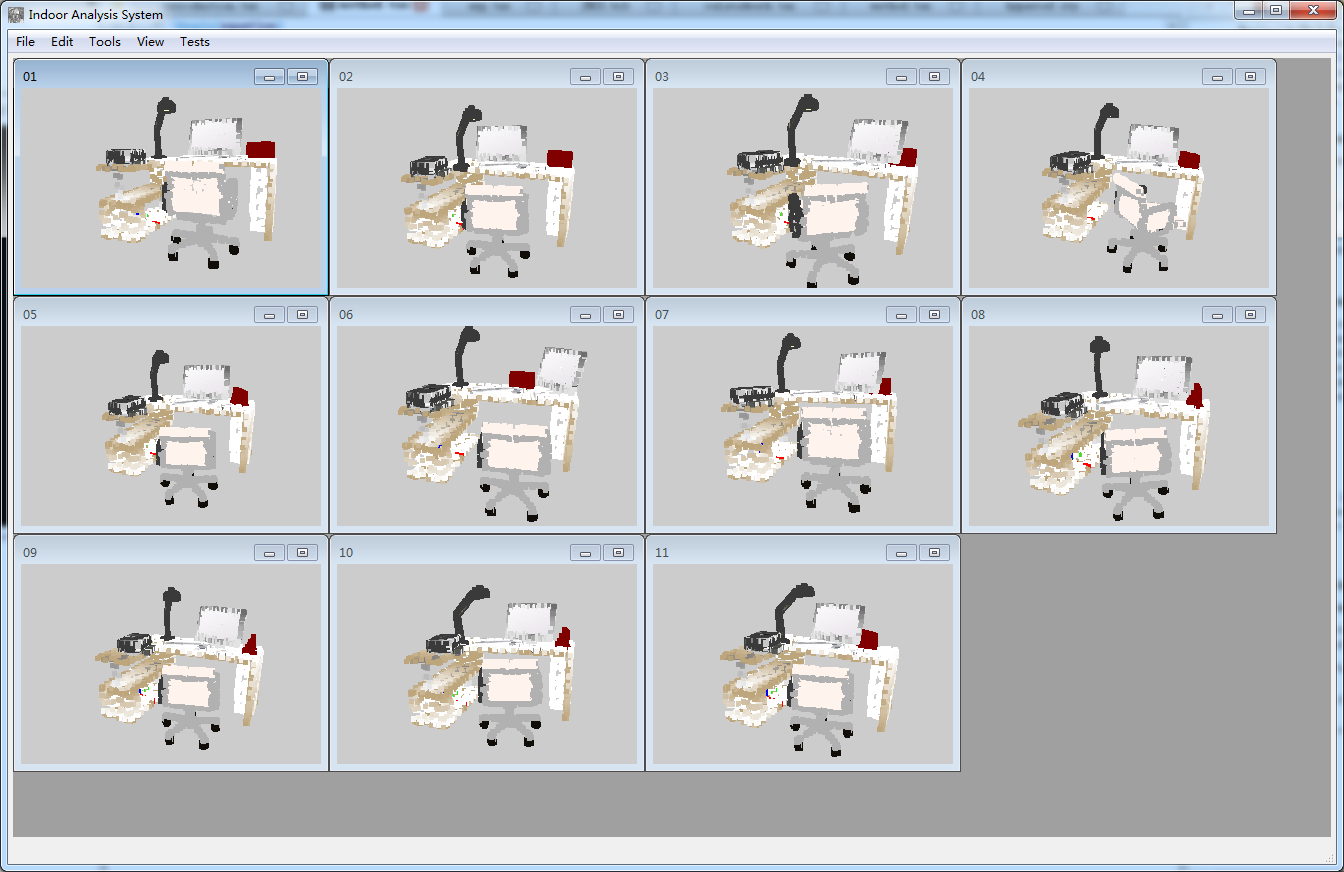
\includegraphics[width=.3\linewidth]{images/interact01.png}
	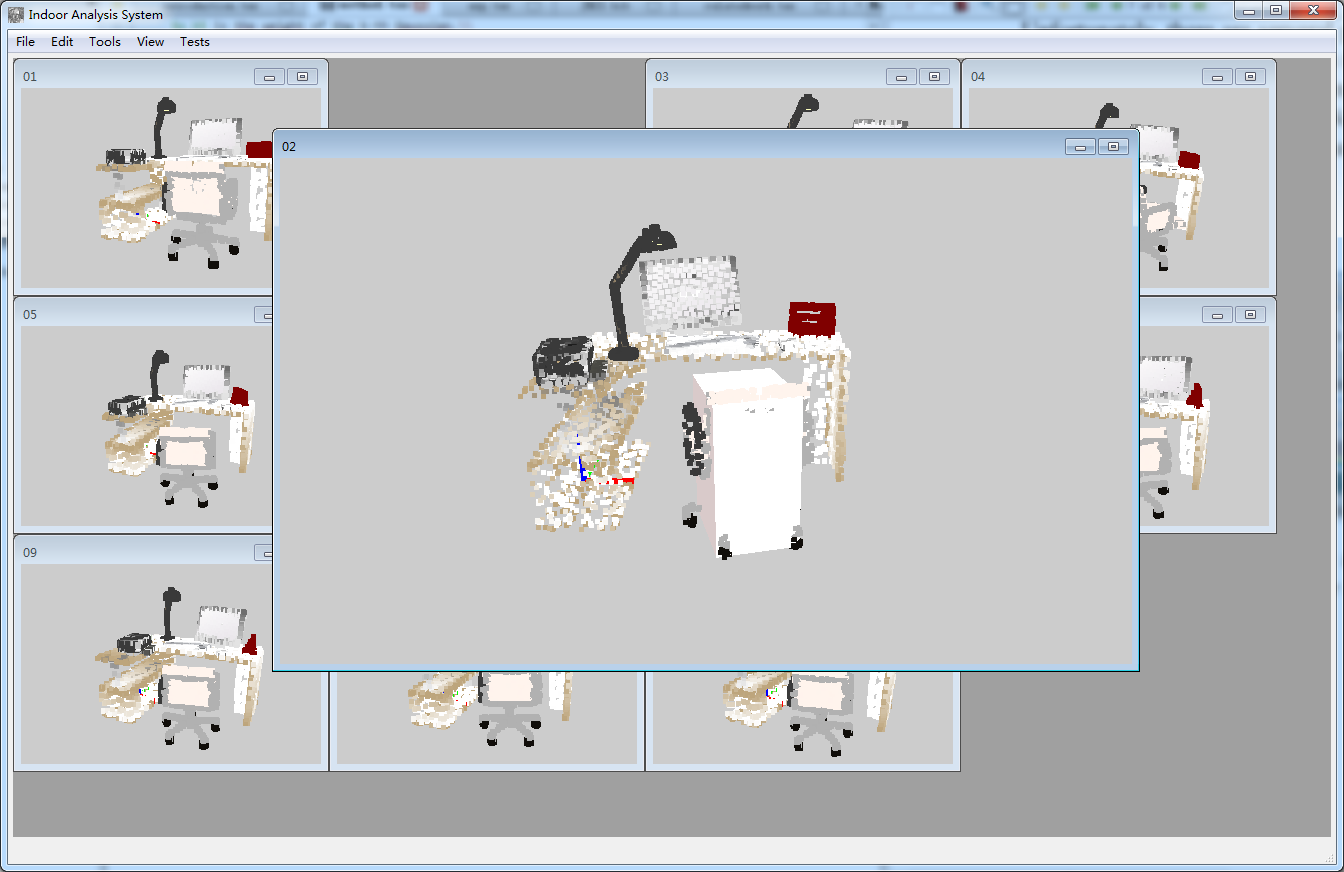
\includegraphics[width=.3\linewidth]{images/interact02.png}
	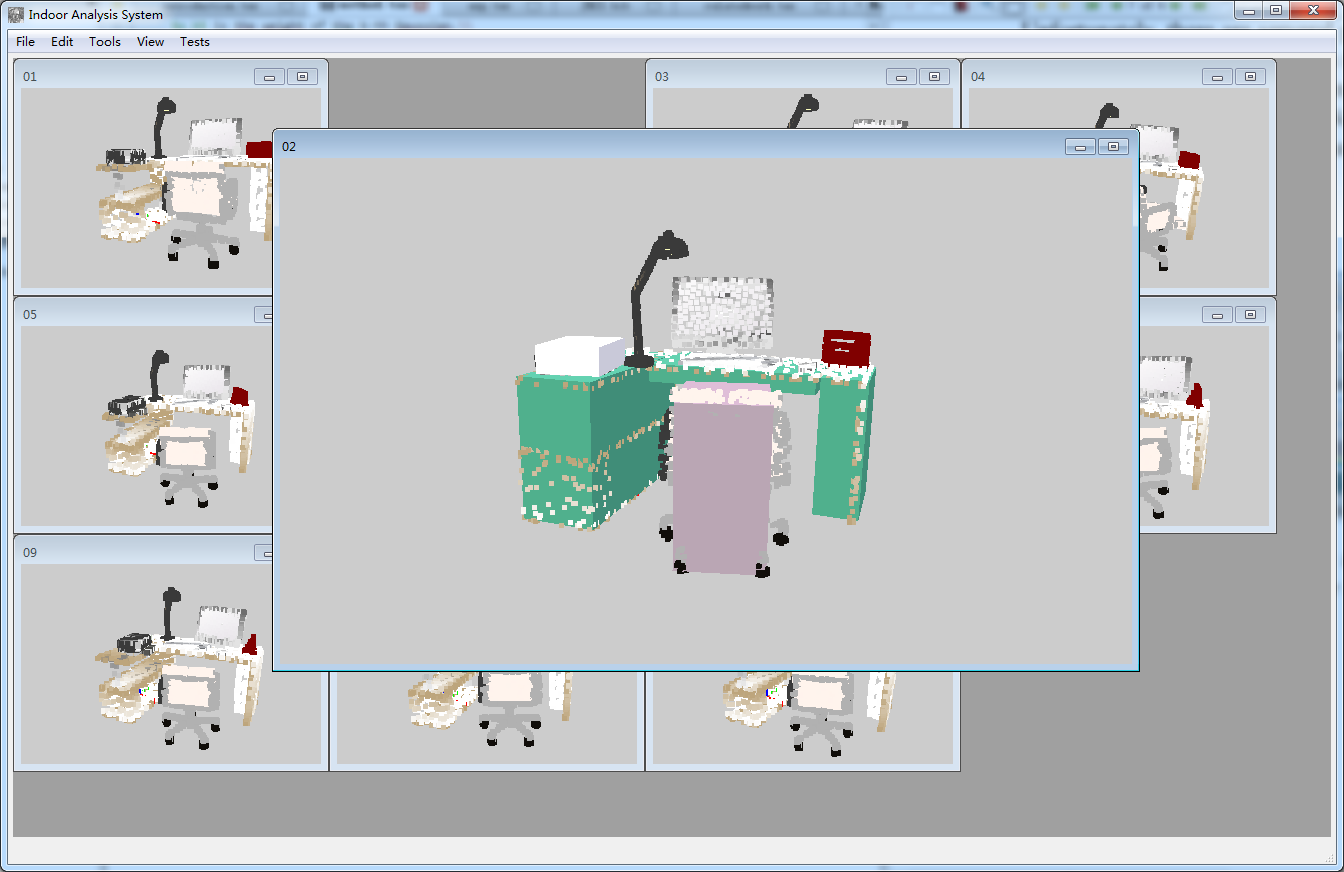
\includegraphics[width=.3\linewidth]{images/interact03.png}
	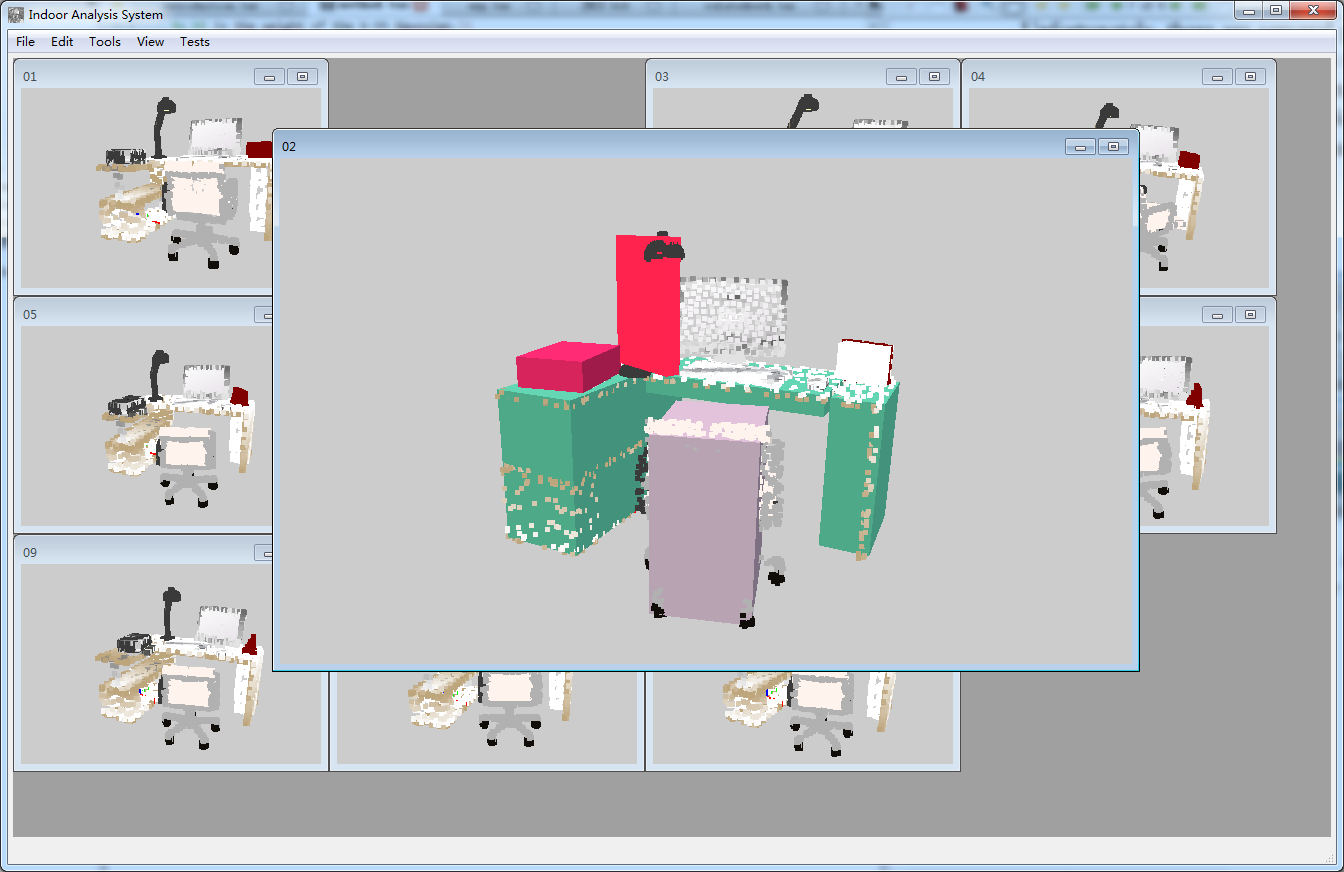
\includegraphics[width=.3\linewidth]{images/interact04.png}
	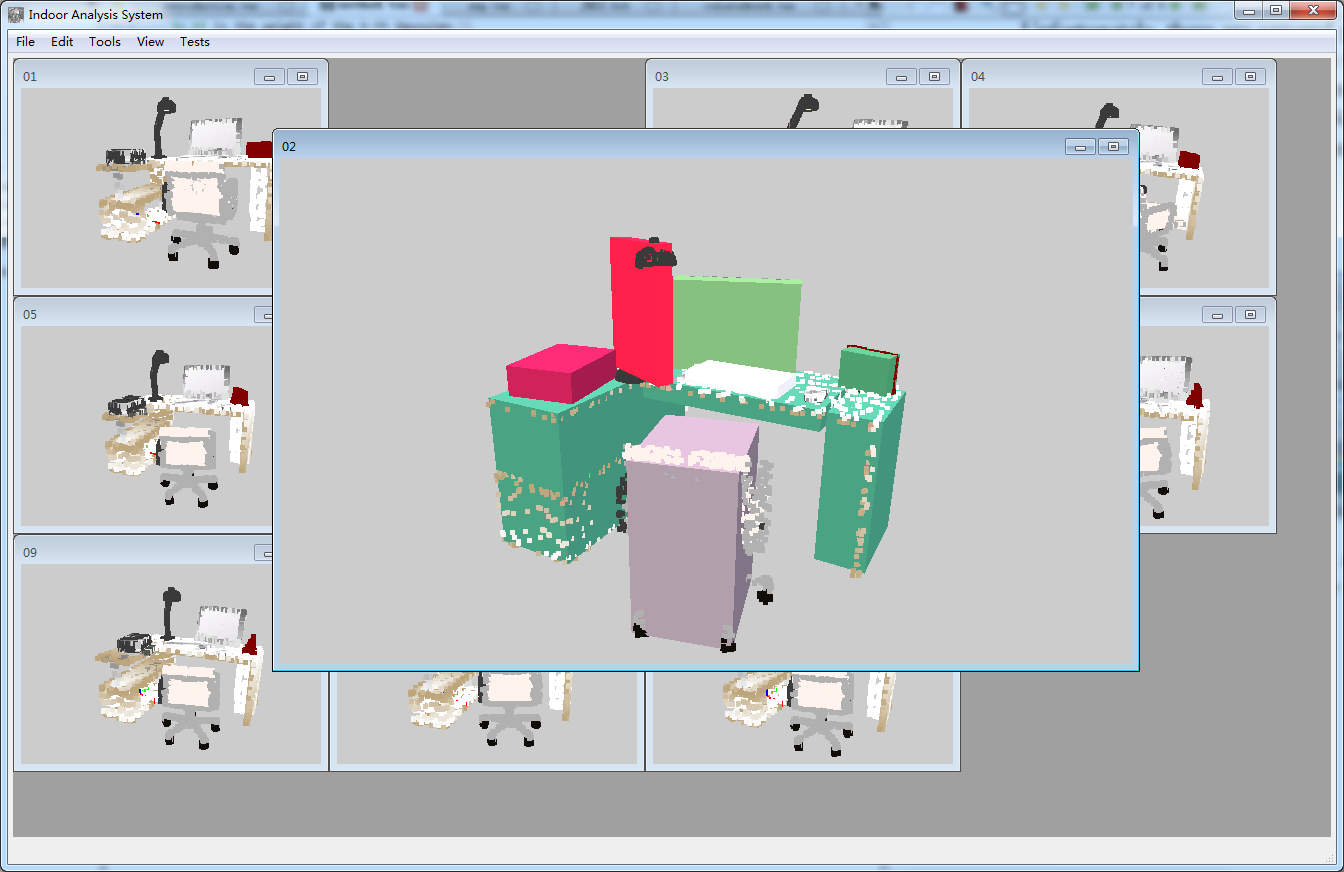
\includegraphics[width=.3\linewidth]{images/interact05.png}
	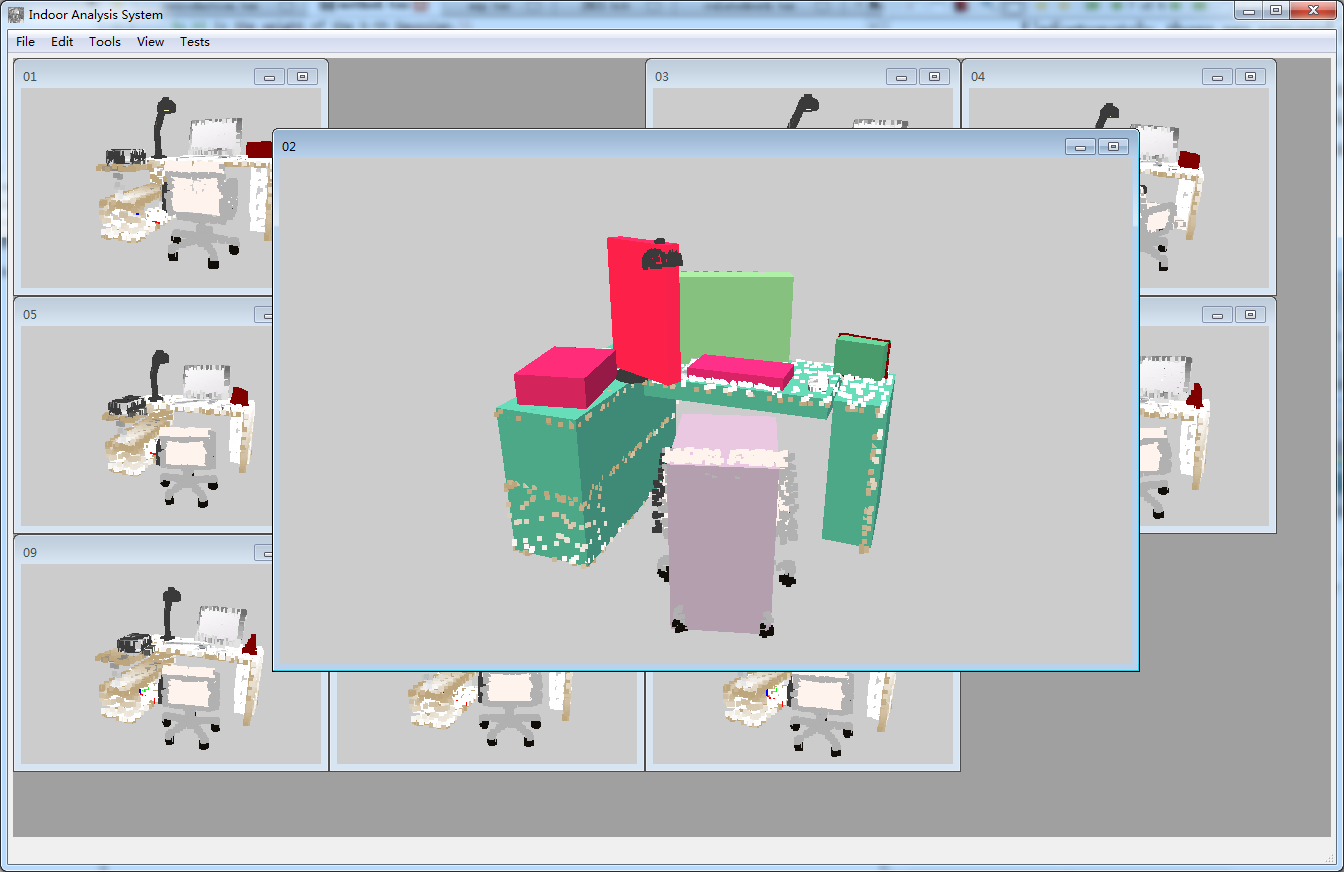
\includegraphics[width=.3\linewidth]{images/interact06.png}
	\caption{\label{fig:interact}
		From the first to the nineth, the nine images show the procedure of interaction:
		the user pick one point set and place boxes in it to indicate the layout for this point set. The box in white is the box currently under editing. The boxes in other colors are boxes placed to represent object layouts. One color represent one object. The interaction allows multiple boxes to represent same object.(e.g. the desk is represented by three boxes in same color)}
\end{figure}
These two paremeters are difficult to be initialized without semantic prior, but with the input of the users we can naturally initialize the $N$ as the number of different color label and the ${K_n}$ as 
\begin{equation}
K_n=\frac{V_n}{\sum V_n}K_{all}
\end{equation}
in which the $V_n$ represent the total volume of the boxes in the n-th color and the $K_{all}$ is initialized as $K_{all}=0.5*median(I_m)$ and $\{I_m\}$ are point numbers of $M$ input point set. This is an emperical choice borrowed from \cite{Evangelidis2014}.\\
The expectation maximizaton framework is easily converge to a local optimal. To cope with this problem we further use this interaction as a soft constraint to guide the optimization. Such constraint is done by 


